\clearpage
\begin{figure}[ht!]
    \centering
    \caption{Feature importance across countries by cluster (non-adjusted)}\label{fig:fig_4_uncorrected}
    \begin{subfigure}[b]{\textwidth}
    \centering
    \caption{Feature importance across countries of cluster A to D}\label{fig:fig_4_1_uncorrected}
    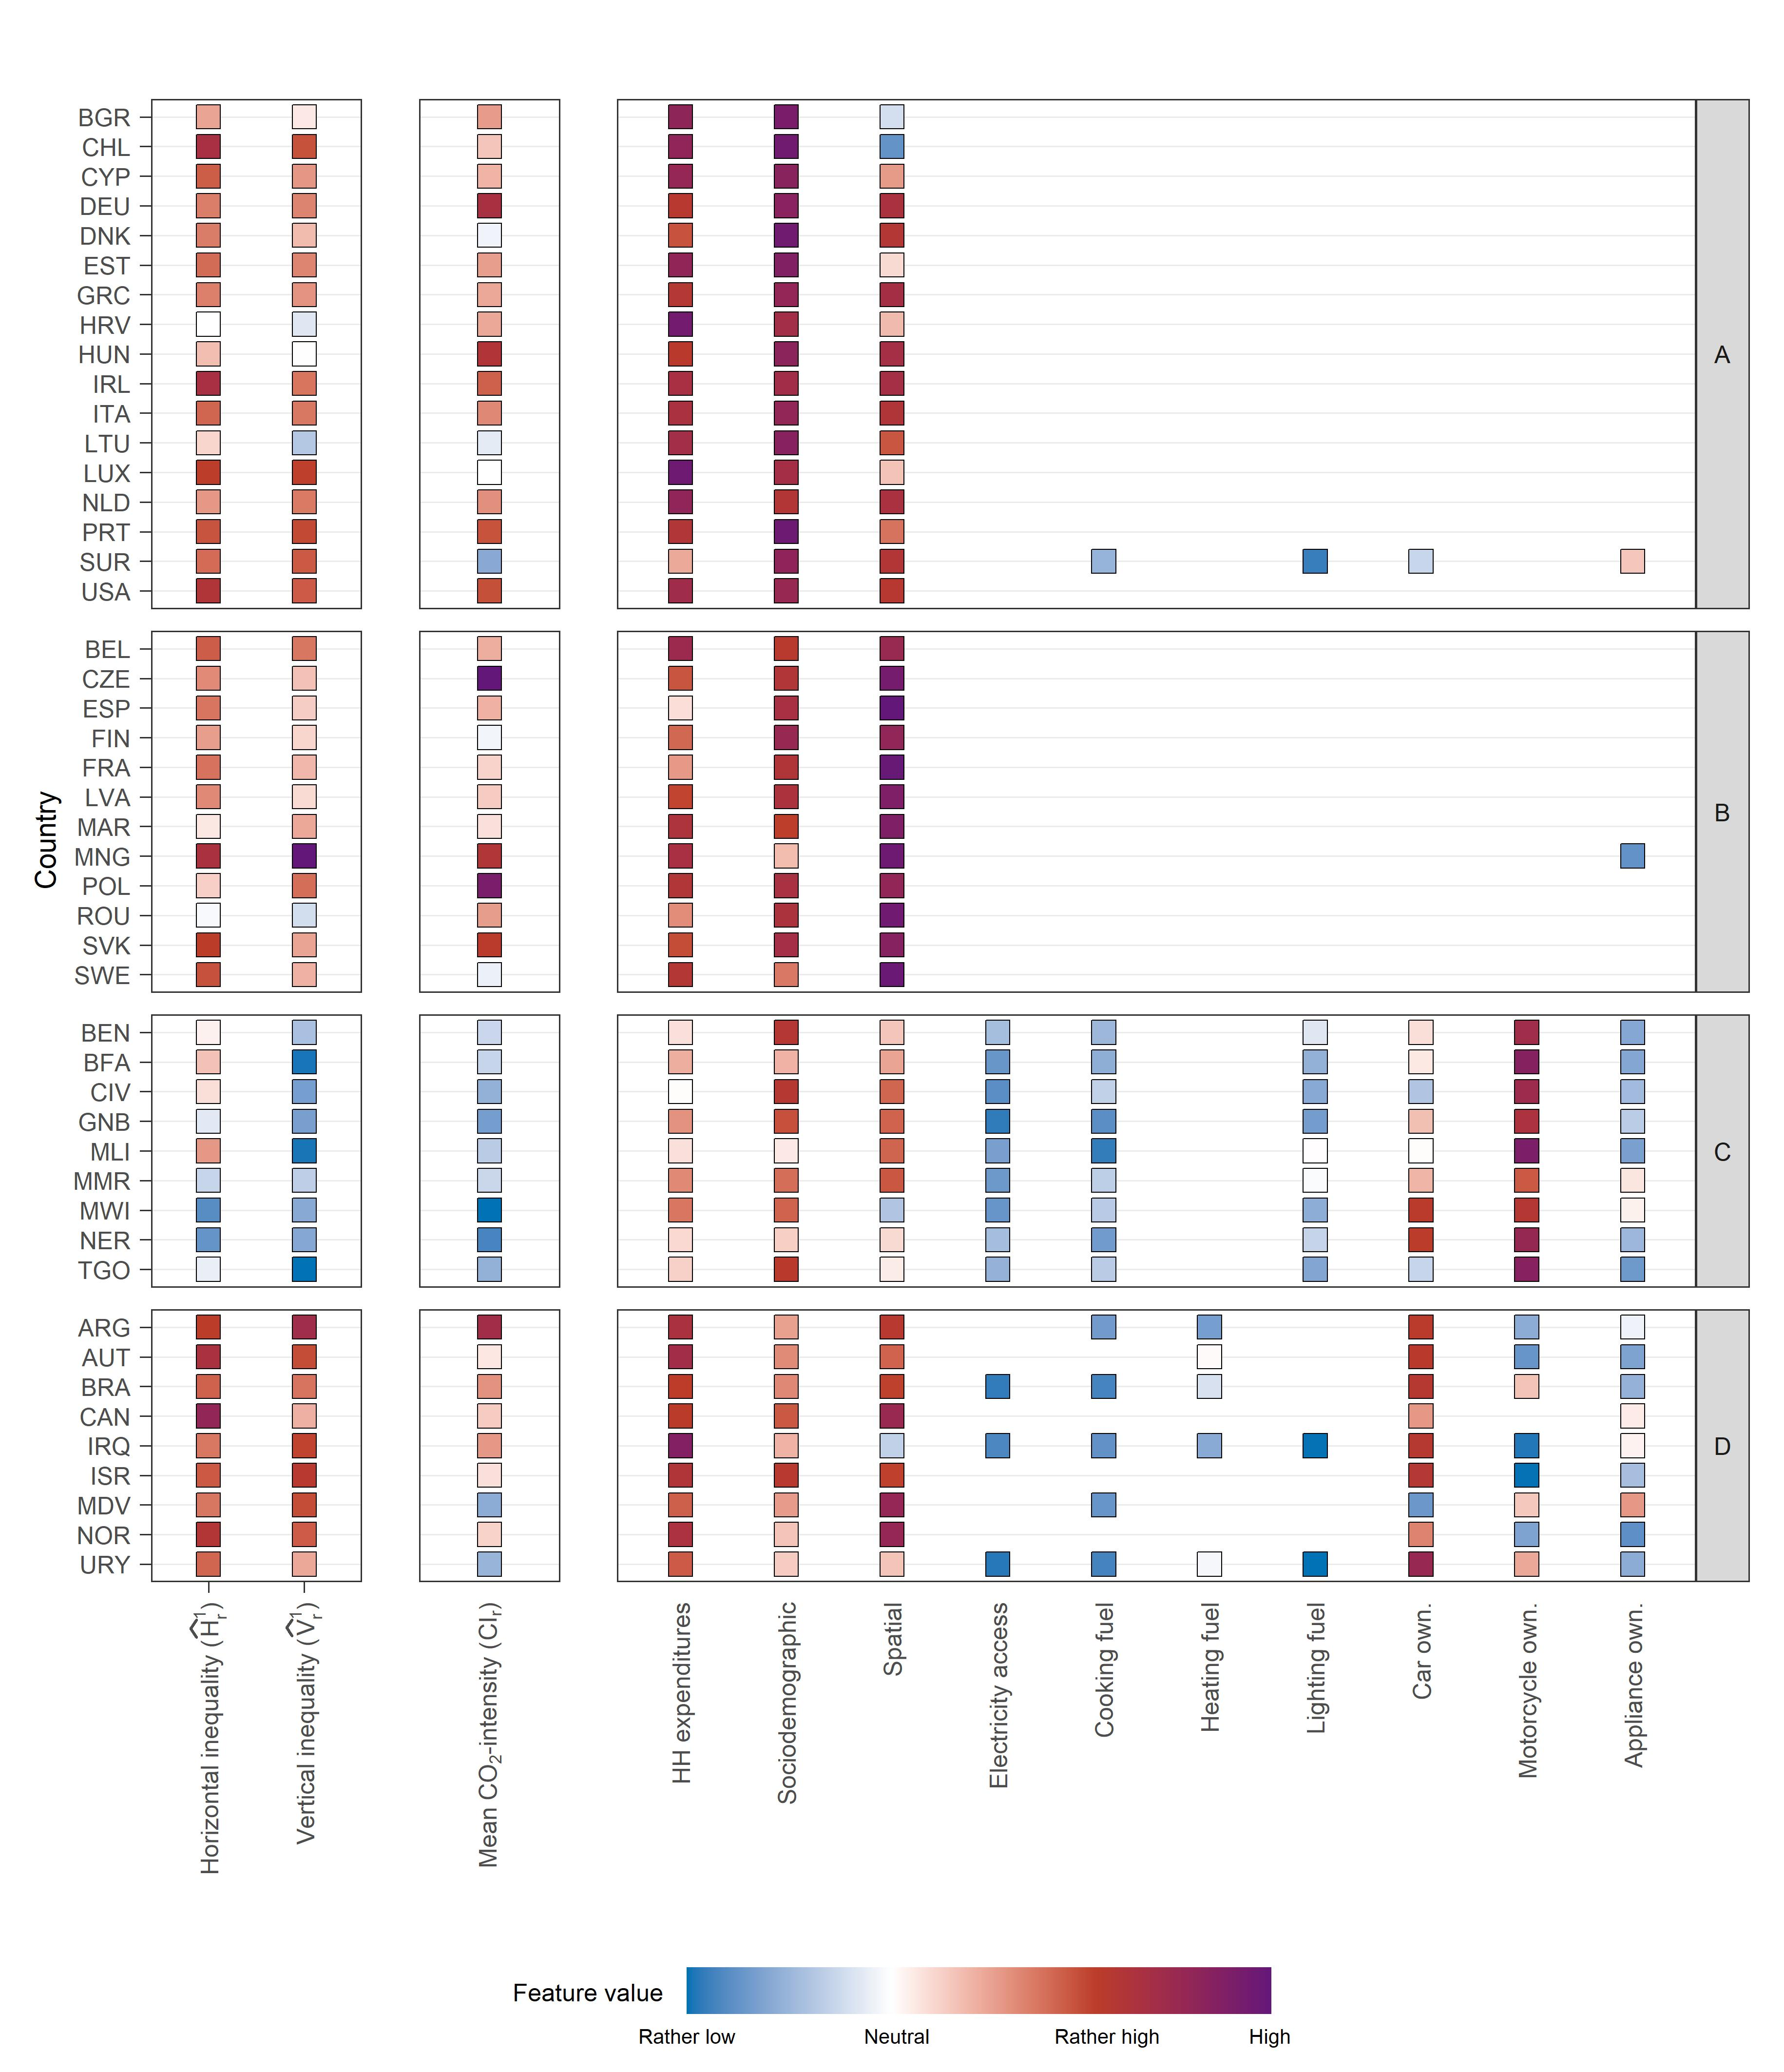
\includegraphics{1_Figures/Figure 4/Figure_4_Uncorrected_1.jpg}
     \begin{subcaption2}
    This figure shows the importance of features (in normalized average absolute SHAP-values) for each country, grouped by country clusters. Blue (red) colors indicate that a feature is relatively less (more) important in a country compared to all other countries and features. 'Sociodemographic' comprises features such as household size, gender, self-identified ethnicity, nationality, religion or language. 'Spatial' comprises features such as state, province, district and urban/rural-identifiers. For horizontal distribution, blue (red) colors indicate a lower (higher) heterogeneity within the poorest quintile compared to the richest quintile. For vertical distribution, blue (red) colors indicate lower (higher) median carbon intensity among the poorest quintile compared to the richest quintile. For average CO$_{2}$-intensity, blue (red) colors indicate a lower (higher) average carbon intensity across all countries. For goodness of fit (R$^{2}$), blue (red) colors indicate a lower (higher) predictive performance compared to other countries. R$^{2}$ is not explicitly included for clustering.
    We assign countries to 13 clusters performing k-means clustering based on \textit{non-adjusted} feature importance values across all features. We also show all values in Table \ref{tab:A10_Uncorrected}.
    \end{subcaption2}
    \end{subfigure}
\end{figure}
\clearpage

\clearpage
\begin{figure}[ht!]\ContinuedFloat
    \centering
    \begin{subfigure}[b]{\textwidth}
    \centering
    \caption{Feature importance across countries of clusters E to M}\label{fig:fig_4_2_uncorrected}
    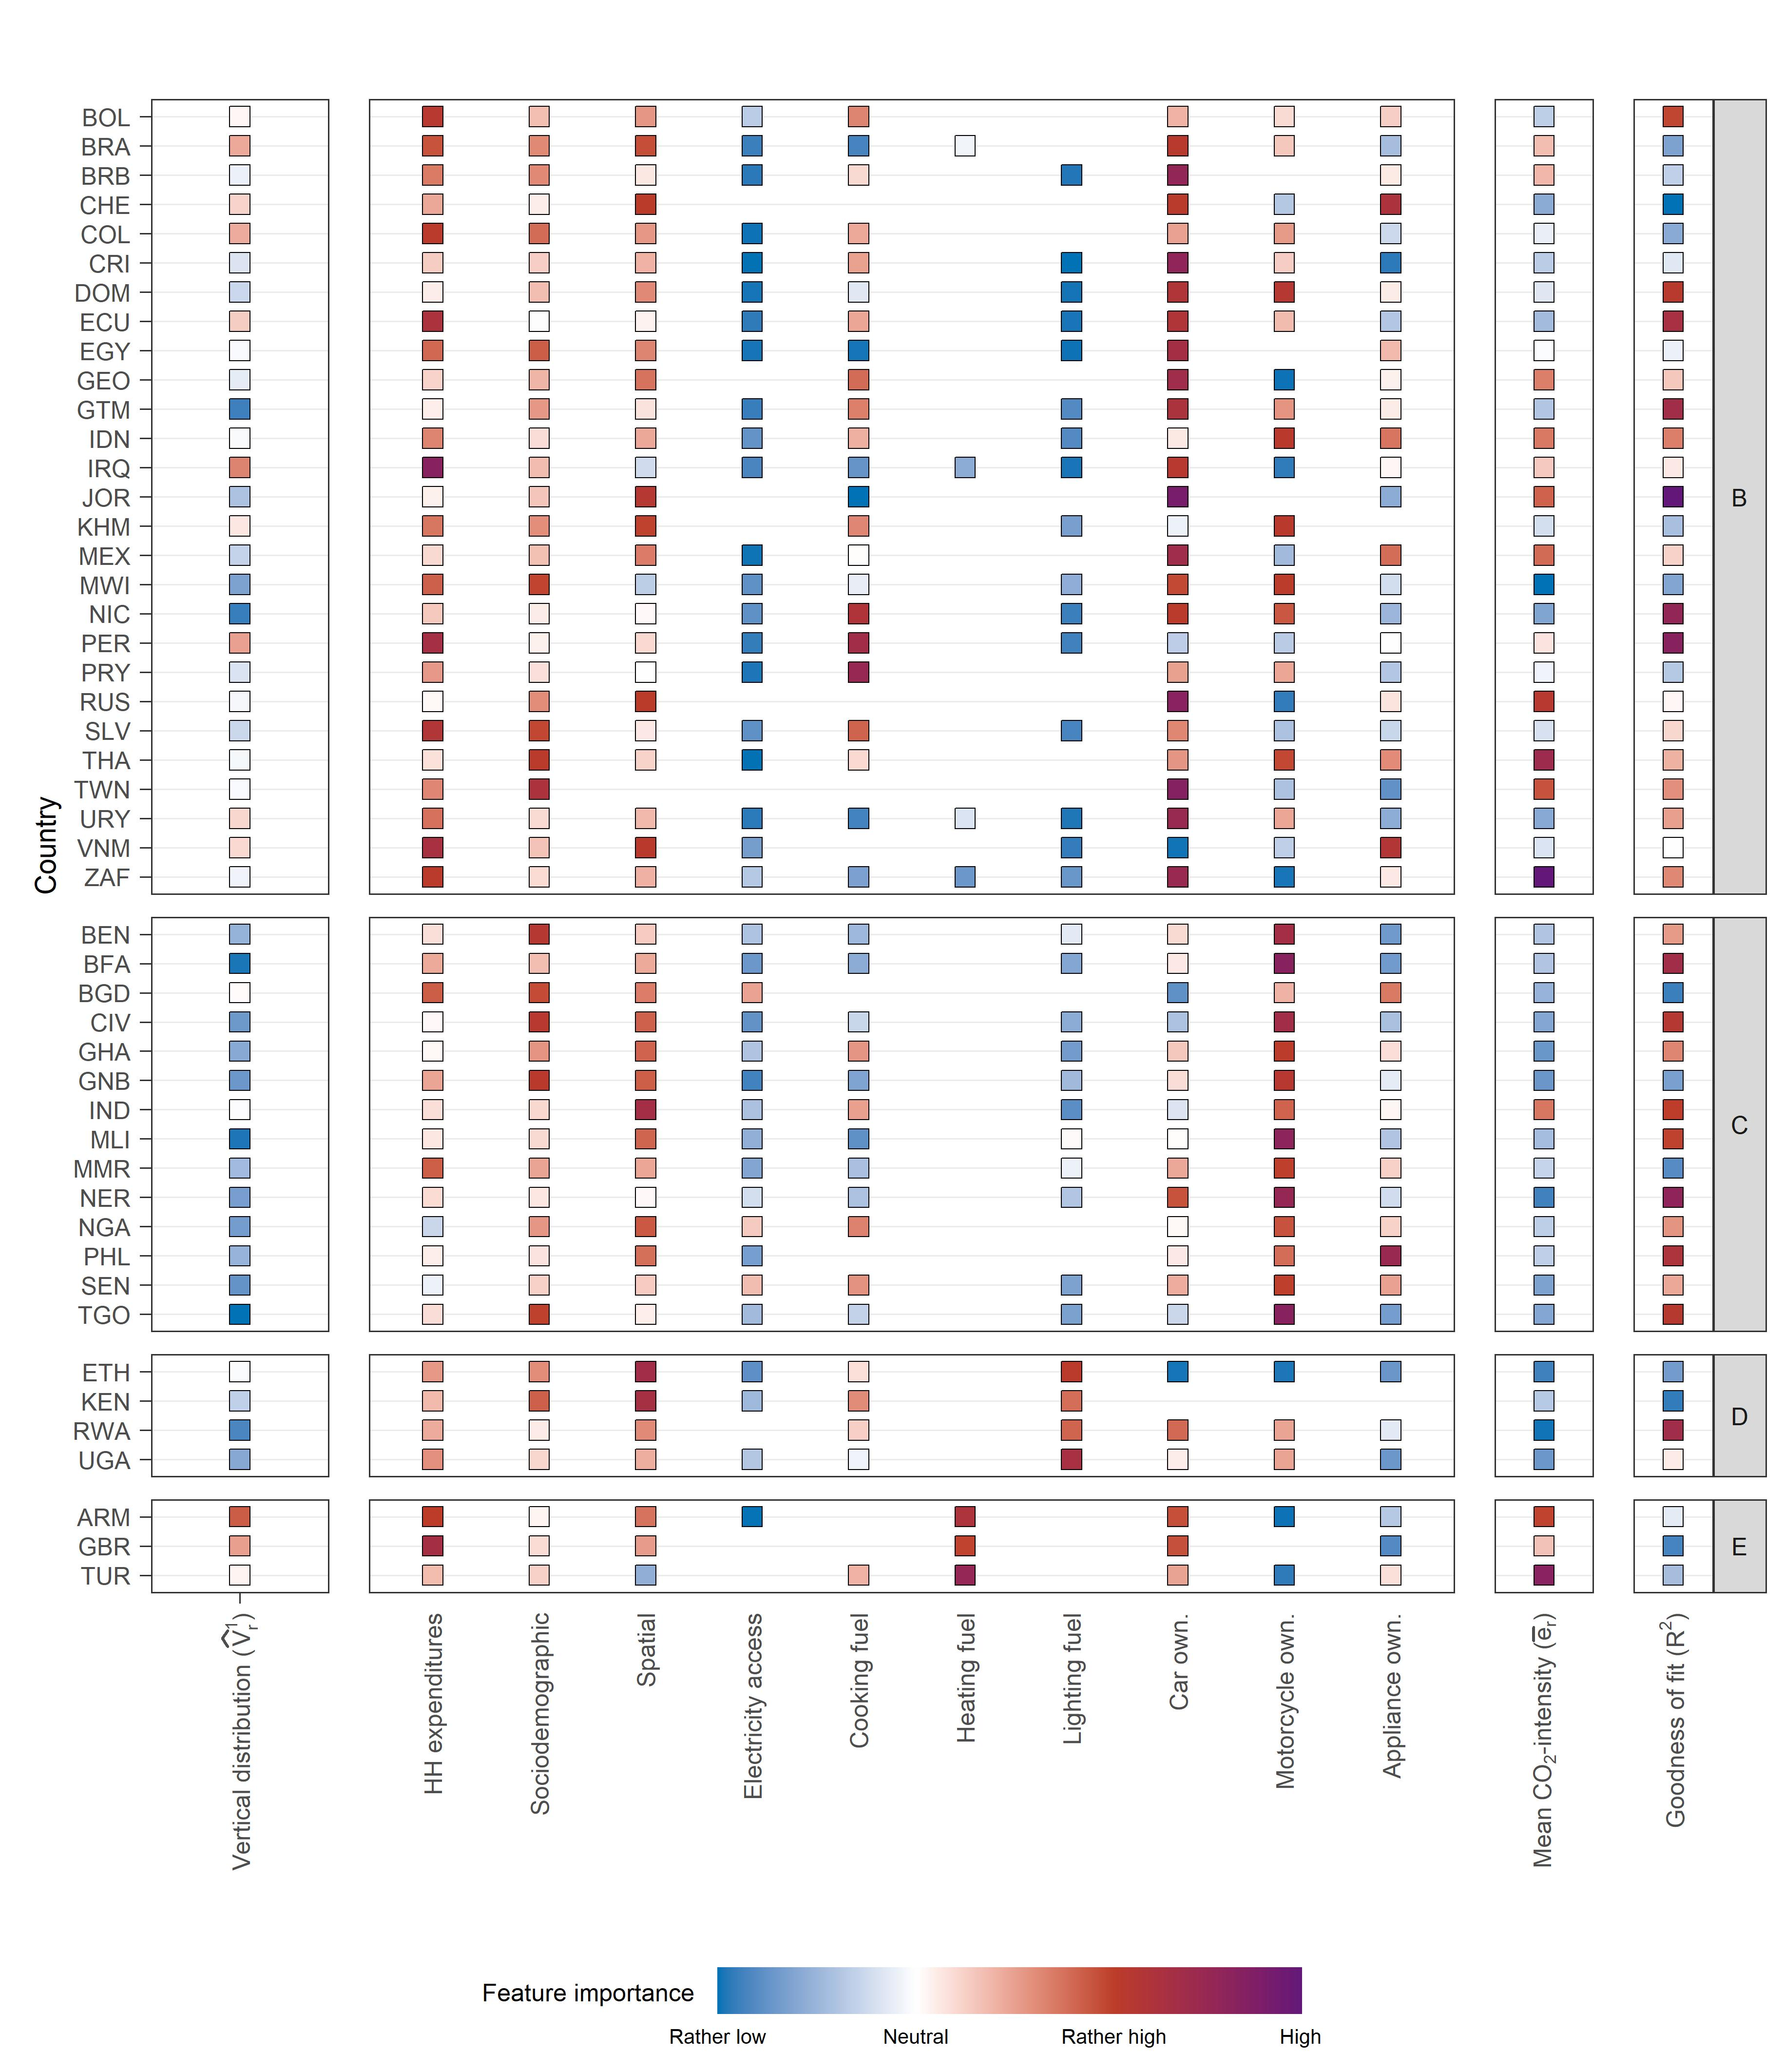
\includegraphics{Figure 4/Figure_4_Uncorrected_2}
    \begin{subcaption2}
    This figure shows the importance of features (in normalized average absolute SHAP-values) for each country, grouped by country clusters. Blue (red) colors indicate that a feature is relatively less (more) important in a country compared to all other countries and features. 'Sociodemographic' comprises features such as household size, gender, self-identified ethnicity, nationality, religion or language. 'Spatial' comprises features such as state, province, district and urban/rural-identifiers. For horizontal distribution, blue (red) colors indicate a lower (higher) heterogeneity within the poorest quintile compared to the richest quintile. For vertical distribution, blue (red) colors indicate lower (higher) median carbon intensity among the poorest quintile compared to the richest quintile. For average CO$_{2}$-intensity, blue (red) colors indicate a lower (higher) average carbon intensity across all countries. For goodness of fit (R$^{2}$), blue (red) colors indicate a lower (higher) predictive performance compared to other countries. R$^{2}$ is not explicitly included for clustering.
    We assign countries to 13 clusters performing k-means clustering based on \textit{non-adjusted} feature importance values across all features. We also show all values in Table \ref{tab:A10_Uncorrected}.
    \end{subcaption2}
    \end{subfigure}
    
\end{figure}
\clearpage